              
% This is based on the LLNCS.DEM the demonstration file of
% the LaTeX macro package from Springer-Verlag
% for Lecture Notes in Computer Science,
% version 2.4 for LaTeX2e as of 16. April 2010
%
% See http://www.springer.com/computer/lncs/lncs+authors?SGWID=0-40209-0-0-0
% for the full guidelines.
%
\documentclass{llncs}
\usepackage{url} % hyperref works too
\usepackage{graphicx}
\usepackage[utf8]{inputenc}
\usepackage{mathtools}
\usepackage{multirow}
\usepackage{mathptmx}

	
\usepackage{caption}


\begin{document}

\title{Poročilo RIS}
%
\titlerunning{Boštjan Bohte}  % abbreviated title (for running head)
%                                     also used for the TOC unless
%                                     \toctitle is used
%
\author{Boštjan Bohte,  Boris Karamatić, Beno Šircelj}
%
\authorrunning{Boštjan Bohte et al.} % abbreviated author list (for running head)
%
%%%% list of authors for the TOC (use if author list has to be modified)
\tocauthor{Boštjan Bohte, Beno Šircelj,  Boris Karamatić}
%
\institute{Ljubljana University, Večna pot 113, Slovenia\\
%\email{bohtebostjan@gmail.com}
}

\maketitle              % typeset the title of the contribution


%

\section{Cilji tretje naloge}
V okviru zadnje naloge pri predmetu RIS smo morali razviti pametni taksi. V laboratoriju je bilo postavljeno majhno "mesto" z "ulicami", "prometnimi znaki", "stavbami" in "osebami". Robot je bil sposoben peljati dve osebi, ki nista istega spola. Taksi je moral poiskati osebo, ki ga je čakala na ulici in jo peljati do želene zgradbe. Prav tako je moral upoštevati tudi cestno prometne predpise, saj so ulice vsebovale znake kot so "stop", "omejitev hitrosti", "obvezno levo" itd. Komunikacija z robotom je morala potekati preko govora. Robot je imel že imel prej določen zemljevid mesta z označenimi ulicami. Lokacije oseb, prometnih znakov in zgradb, pa je moral zaznati sam. V nalogi smo morali implementirati zaznavanje in prepoznavanje obrazov, prepoznavanje in upoštevanje prometnih znakov, navigacija po mestu, iskanje oseb ter stavb.




\section{Metode}


\subsection{Prepoznavanje govora}
Za implementacijo govora smo uporabili android aplikacijo, ki smo jo dobili s strani predmeta. V vozlišču 'talk' smo se na to prijavili na temo '/command', kamor smo pošiljali zaznan govor z aplikacijo. Dobljeni string smo na to razbili na posamezne besede, jih spremenili v male črke ter jih shranili v tabelo. Na osnovi prve besede smo določili ali moramo koga pobrati ('find') ali koga kam odpeljati ('take'). Na osnovi druge besede smo določili koga in na osnovi četrte kam. Ukazi so bili oblike 'Find Matthew on green street' oz. 'Take Matthew to yellow hotel'. Po vsakem ukazu je robot še zahteval potrditev, da je ukaz res pravilno razumel.
Za robustifikacijo govora smo implementirali Levenshteinovo razdaljo, ki deluje tako, da primerja med seboj dva stringa in vrne število potrebnih operacij, tj. koliko črk bi bilo potrebno zamenjati, odstraniti ali dodati, da bi prvi string postal enak drugemu. Prav tako pa smo dodali tudi naš slovar besed, ki smo ga gradili sproti, med testiranjem.


\subsection{Prepoznavanje znakov in obrazov}
Prepoznavanje znakov in obrazov je sestavljeno iz dveh delov, klasifikacijski model in ustvarjanje učne množice. Slednji se uporablja samo za pripravo klasifikacijskega modela in je nato neaktiven čez celotni proces, drugi del pa omogoča razpoznavanje različnih znakov ali obrazov in je vedno aktiven. Ker je teren zaprt prostor in so skoraj idealni pogoji, ni bilo potrebno narediti velike učne množice. 

\subsubsection{Ustvarjanje učne množice znakov:} 

Prijavimo se na temo 'traffic\underline{ }signs', katero vozlišče je bilo implementirano s strani predmeta in iz nje pridobivamo podatke o detektiranem znaku. Zanima nas samo velikost in pozicija znaka na sliki. Iz slike izluščimo znak in ga nastavimo na velikost 50x50 pikslov. Znaku nato izenačimo histogram za vsak barvni kanal R,G,B, da dobi boljšo odpornost na spremembe svetlosti v prostoru. Znak nato shranimo z oznako v posebno mapo, kjer bo služil za učno množico modela. Naredili smo približno 30 učnih primerov za vsak znak, ker se je izkazalo, da je to zadostno število in je s tem bilo tudi učenje krajše. 

\subsubsection{Prepoznavanje znakov:}
Pri prepoznavanju znakov ustvarimo najprej klasifikacijski model. Za to nalogo smo določili, da bo bil to model k najbljižjih sosedov, ker je prosto dostopen v knjižnjici OpenCV. Iz mape kjer so označene slike znakov, preberemo celotno sliko kot matriko, jo sploščimo v vektor in podamo modelu kot učni primer. Učenje je hitro, saj rabi malo učnih primerov zato se to naredi vsakič, ob zagonu procesa. 

Prijavimo se na temo 'traffic\underline{ }signs'(detektor znakov), kjer nas zanima pozicija in velikost znaka. Enako kot pri učenju izrežemo ven znak, ga nastavimo na velikosti 50x50 pikslov in na vseh barvnih kanalih RGB izenačimo histogram. Matriko spremenimo v vektor in podamo na vhod modela. Model nam vrne razdaljo in napovedan znak. Razdalja lahko služi kot neko verjetje, večja kot je, manjša je zanesljivost te napovedi. Da proces vrne kateri znak je prepoznal, mora bit razdalja manjša od nastavljenega praga in znak mora biti v kratkem intervalu časa zaznan vsaj petkrat. Detektor pošilja detektirane znake okoli 10x na sekundo, kar pomeni, da bo detektiran znak prepoznal v približno 0.5 sekundah. Čas je ključnega pomena, saj bi lahko v daljšem zamiku zgrešil znak. Za večjo robustnost se zato bolj zanašamo na prag razdalje. Med testiranjem model ni napovedal nobenih nepravilnih prepoznav, lahko pa je zgrešil znak zaradi premalo detekcij. 

\subsubsection{Ustvarjanje učne množice obrazov:}
Prijavimo se na temo 'faces', katero vozlišče je bilo implementirano s strani predmeta in iz nje pridobivamo podatke o detektiranem obrazu. Zanima nas lokacija in velikost obraza na sliki. Iz slike izrežemo detektiran obraz in spremenimo v sivinsko sliko. Sliki nato še izenačimo histogram, da je bolj odporna na spremembe svetlobe. Izrezek slike nato shranimo pod oznako obraza, ki bo služil kot učni primer. Za vsako obraz smo naredili približno 20 učnih primerov. 

\subsubsection{Prepoznavanje obrazov:}
Za prepoznavanje obraza uporabimo model LBPH, ki je implementiran v OpenCV knjižnjici in je prosto dostopen. Za vhod rabi sivinske slike obrazov, velikost matrike pa ni potrebno da je enaka, zato je učenje modela enostavno. Samo preberemo iz mape vse shranjene slike obrazov in jih uporabimo kot učno množico. Zaradi majhne učne množice tudi to učenje traja kratek čas, zato se učenje izvaja ob vsakem zagonu procesa.

Prijavimo se na temo 'faces' (detektor obrazov) in nas zanima pozicija in velikost detektiranega obraza. Iz teh podatkov izrežemo obraz iz slike, izrezek pretvorimo v sivinsko sliko in izenačimo histogram. Obdelano sliko vstavimo v naučeni model in nam vrne napoved in verjetnost te napovedi. Večja je verjetnost, bolj zanesliva je napoved. Tudi tokrat uporabimo prag za verjetnost in število detekcij v danem intervalu. Ker iskanje obrazov ni tako časovno pomembno, ga mora model prepoznati vsaj 10x, kjer mora med vsako prepoznavo miniti manj kot 0.2 sekundi, da pošlje prepoznan obraz naprej. Med testiranjem model ni napovedal nobenih nepravilnih prepoznav. 


\subsection{Upoštevanje znakov}
\subsubsection{Omejitev hitrosti in stop:}
Oba znaka sta bila implementirana v istem vozlišču. V tem vozlišču poslušamo kaj objavlja detektor znakov na temi '/sign'. Tako dobimo marker, ki vsebuje za vsak znak unikaten id po katerem vemo kateri znak je bil zaznan. Pri prejetju detekcije spremenimo speed\underline{ }lim\underline{ }v parameter v /navigation\underline{ }velocity\underline{ }smoother z dinamično nastavitvijo. 
system("rosrun dynamic\underline{ }reconfigure dynparam set /navigation\underline{ }velocity\underline{ }smoother speed\underline{ }lim\underline{ }v 0");
Pri čemer je hitrost 0 za zaznan znak stop in 0.7 za zaznan znak omejitev hitrosti. Po nekaj sekundah vrnemo hitrost nazaj na začetno. Da se večkrat ne ustavi pred istim znakom imamo še en sleep(30), ki preprečuje detekcijo istega znaka v naslednjih 30 sekundah.
\subsubsection{Obvezno potrobi:}
Podobno kot pri Stop-u poslušamo na temi '/sign'. Ko prejmemo marker z id-jem, ki ustreza znaku za stop zaženemo play.py, ki preko sound\underline{ }play-a predvaja naš zvok.
int i = system("rosrun sound\underline{ }play play.py /home/team\underline{ }zeta/catkin\underline{ }ws/src/horn.wav");
\subsubsection{Enosmerna:}
Enosmerno ulico smo implementirali, tako, da smo uporabili tri zemljevide. Sredinski je brez omejitev, ostala dva pa imata pregrado pri znaku napačna smer.
Naloga tega vozlišča je, da ob detekciji enosmerne, prestavi robota v ustrezno mapo. Ko vozlišče prejme marker, ki ima id, ki ustreza znakoma obvezno levo ali napačna smer, izračuna v katero mapo mora prestaviti položaj robota. To izračuna tako, da posluša temo '/amcl\underline{ }pose' in s tem dobim trenutni položaj robota. Na osnovi tega izračuna, če se nahaja v delu mape iz koder se vidi znak v zeleni ali znak v rumeni ulici. Ko izračunamo kam moremo prestaviti robota pošljemo nov položaj na temo '/inicialpose'. Ker so cilji še vedno v stari mapi se pošlje še ukaz za posodobitev ciljev vozlišču 'pathSetter'.
Da bi ob premiku robota v novo mapo preprečili njegovo zgubljanje in vrtenje v krogu, ko poskuša priti do starega cilja, ki se še vedno nahaja v prejšnji mapi, mu trenutni cilj ob teleportaciji takoj še prekinemo. To storimo tako, da nastavimo cilj na robotovo trenutno lokacijo. V vozlišču pathSetter se vsak cilj, ki je bil prekinjen pošlje še enkrat, ampak tokrat z novimi koordinatami. Ko pridemo do cilja vrnemo robota s podobnim postopkom nazaj v sredinski zemljevid. Zemljevid je prikazan na sliki~\ref{div}.



\subsection{Prepoznavanje cilindrov}
Za prepoznavanje in detekcijo cilindorv, smo uporabili knjižnjico pointcloudlibrary. Prijavili smo se na temo 'input', ki nam je dajala podatke iz 3D okolja v pcl formatu. Ker je v enem posnetku veliko podatkov in je s tem iskanje cilindrov počasen proces, smo morali odstraniti čim več točk iz točkovnega oblaka. Najprej smo odstranili točke, ki so od rumbe oddaljene več kot 2 metra po  x in y osi in 1 meter po z osi. Odstranili smo tudi vse točke, ki so pripadali ravnini in nato začeli iskati cilinder. Če cilinder prepozna, pošljemo vse njegove barvne točke v funckijo za preverjanje barve cilindra. Prepoznani cilinder prikazuje slika~\ref{cil}. Tam preberemo vse barve točk in jih povprečimo za vsako barvo posebej (R,G,B). RGB prostor barve spremenimo v HSV in tam po Hue vrednosti iščemo barve cilindorv, ki so v mapi. Če nobena barva ne ustreza, cilinder zavržemo. Iz oblaka točk cilindra poiščemo centroide za vsako os in njihove min in max vrednosti koordinat. S tem dobimo obliko najdenega cilindra in če ni podobna obliki naših cilindrov, ga zavržemo. S tem smo izločili večino šuma in ko pošljemo marker na neko temo, velja ta marker za veljavni cilinder. Kljub temu pride do morebitnih napak, zato se to temo posluša samo takrat, ko iščemo cilindre in najdeni cilinder mora biti iskane barve. 



\subsection{Premikanje po prostoru}
Za premikanje smo na vsaki ulici določili statične točke, ki so služile kot cilji robotu. Robot se je po teh točkah premikal in tako iskal osebe ali hotele.

\section{Povezovanje vozlišč med seboj}

\subsubsection{TALK:} Vozlišče 'talk' je sprejemalo govor. Prav tako je preverjalo dovoljenost zahtevanih operacij (če želimo koga kam odpeljati, preveri če je ta oseba res v taksiju; če hočemo dodati koga v taksi, preveri, da ni v njemu že kaka druga oseba tega spola, … ). Prav tako je tudi hranilo stanje taksija, tj. kdo se trenutno nahaja v taksiju. To vozlišče je na to sporočalo vozlišču 'pathSetter' ali naj išče osebo ali hotel, katero osebo ali hotel ter na kateri ulici.
\subsubsection{PATHSETTER:} Vozlišče 'pathSetter' je na to nastavilo pravilne v naprej določene cilje, kam naj se robot odpelje ter sporočilo vozlišču 'approach' koga oz. kaj iščemo.
\subsubsection{APPROACH:} Vozlišče 'approach' je od 'pathSetterja' dobilo informacijo kaj naj išče, in hkrati je poslušalo kaj objavljata detektor obrazov in hotelov. Ko je detektiralo iskan objekt, je 'pathSetterju' sporočilo, da lahko ustavi iskanje, ter nato izračunalo kam naj se približa. Ko smo se približali hotelu je vozlišču 'talk' tudi sporočilo koga naj odstrani iz taksija.
\subsubsection{HORN:} Vozlišče 'horn' je poslušalo kaj objavlja detektor prometnih znakov. Ko je zaznalo znak za potrobiti je potrobil. Dodali smo, da se lahko to zgodi samo vsakih 30 sekund.
\subsubsection{SLOW:} Vozlišče 'slow' je poslušalo kaj objavlja detektor prometnih znakov. Ko je zaznalo znak za počasi je znižal hitrost za 5 sekund. Ko je zaznalo znak stop, pa je znižal hitrost na nič za 2 sekundi.
\subsubsection{TELEPORT:} Vozlišče 'teleport' je poslušalo kaj objavlja detektor prometnih znakov. Ko je zaznalo znak za enosmerno ali obvezno levo, je preveril kje se robot trenutno nahaja ter ga teleportiralo v pravilno mapo. Vozlišču 'pathSetter' je ob teleportaciji sporočil v katero mapo je premaknil robota, tako da je slednji lahko posodobil svoje cilje.
\subsubsection{FACES:} Vozlišče 'faces' je skrbelo za detekcijo in prepoznavanje obrazov. Ko je prepoznalo obraz je to sporočilo na temo '/foundFace'.
ZNAKI Vozlišče 'znaki' je skrbelo za detekcijo in prepoznavanje znakov. Ko je prepoznalo znak je to sporočilo na temo '/sign'.
\subsubsection{CLUSTER:} Vozlišče 'cluster' skrbelo za detekcijo in prepoznavanje cilindrov. Ko je prepoznalo cilinder je to sporočilo na temo '/hotel'.







\section{Hardware in software problemi}
\subsubsection{COSTMAP:} Eden izmed problemov, ki smo ga imeli je bil, da je robot obtičal sredi ulice in sporočal, da ne more doseči svojega cilja, čeprav je bila pot do tam prosta. Dokler nismo končno ugotovili, da je pravzaprav kriv costmap, nam je to povzročilo veliko težav, saj nismo vedeli kdo je krivec.
Costmap zidove, omarice in ostale ovire napihne in s tem prepreči, da bi se robot vanje zabil. Zelena in rumena ulica sta bile na določenih delih zelo ozke in ko se je costmap tam napihnil se je včasih zgodilo, da je robot mislil, da ne more iti tam mimo. Ko smo ugotovili, da je krivec costmap, smo zmanjšali njegovo napihnjenost, s tem smo nekoliko izboljšali premikanje robota, a sedaj se je vsake toliko zabil v kakšno omarico. 
\subsubsection{WAITFORTRANSFORM:} Funkcija 'WaitForTransform()', ki čaka, dokler ni pretvorba iz okolja robota v okolje mape na voljo je vedno trajala 1 sekundo. Posledično je ustvarjala ozko grlo v programu. V tretjem tekmovanju smo se temu sicer izognili tako, da smo detekcijo objektov objavili samo takrat, ko smo bili 100\% prepričani, da smo našli obraz oziroma hotel. S tem smo bili prisiljeni čakati eno sekundo samo takrat, ko smo se želeli približati. 
\subsubsection{ros::Time::now():} Ko smo dobili lokacijo obraza oz. hotela glede na robota in smo želeli to lokacijo pretvoriti v okolje mape, bi morali uporabiti čas, ki se je nahajal v headerju markerja. Ko smo uporabili ta čas smo vedno dobili napako 'Extrapolation would require a lookup into the future', katerega nismo mogli nikakor odpraviti. Ko smo spraševali druge ekipe, so imele tudi one enake težave. Posledično, če detektiramo obraz med premikanjem in ga pretvorimo v prostor mape, ga bo zaradi premikanja robota pretvorilo narobe. Ker problema nismo mogli odpraviti, smo bili prisiljeni ga zaobiti ter računati lokacijo obrazov oz. hotelov samo takrat, ko je bil robot pri miru. Zato smo tudi vsak obraz gledali po 2 sekundi. Tako smo lahko izračunali lokacijo za se približati pravilno, saj je robot bil pri miru.
\subsubsection{Speech client:} Speech client, ki je povezal android aplikacijo z robotom se včasih ni želel zagnati iz prve in je bilo potrebno njegovo vozlišče večkrat pognati.
\subsubsection{Laptop baterija:} Čeprav smo imeli prenosnik na polnilniku vedno, ko se nismo vozili naokoli, se je vedno zgodilo, da smo prej ali slej ostali brez baterije, saj se enostavno prazni hitreje, kot se lahko polni. Kot predlog za izboljšanje bi bilo dobro, če bi se kupilo več baterij, katero bi se na to, ko se sprazni lahko zamenjalo enako kot pri robotu.
\subsubsection{Sesanje:} Včasih med prižiganjem robota se zgodi, da se zažene v načinu za sesanje. Enkrat, ko je v tem načinu pa se zna zgoditi, da ti vzame veliko časa preden ti ga uspe resetirati, da začne ponovno delovati kot mora.
\subsubsection{Dokumentacija:} Nekateri deli ROS-a so zelo slabo dokumentirani, ali pa dokumentacije sploh nimajo.




\begin{figure}
  \centering
    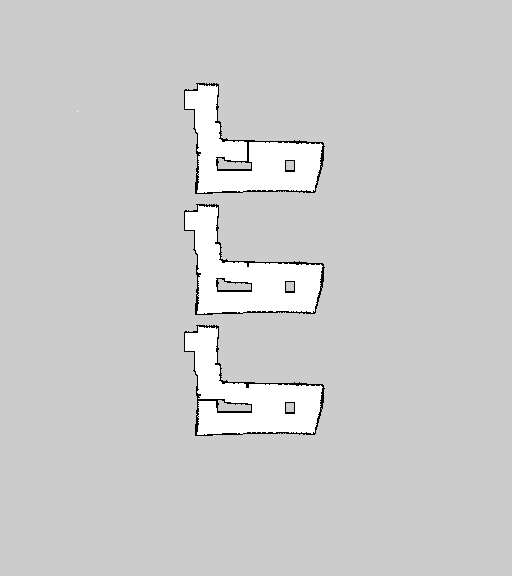
\includegraphics[width=1\textwidth]{aze.png}
  \caption{Slika prikazuje zgrajeno mapo sestavljeno iz treh stanj.}
  \label{div}
\end{figure}


\begin{figure}
  \centering
    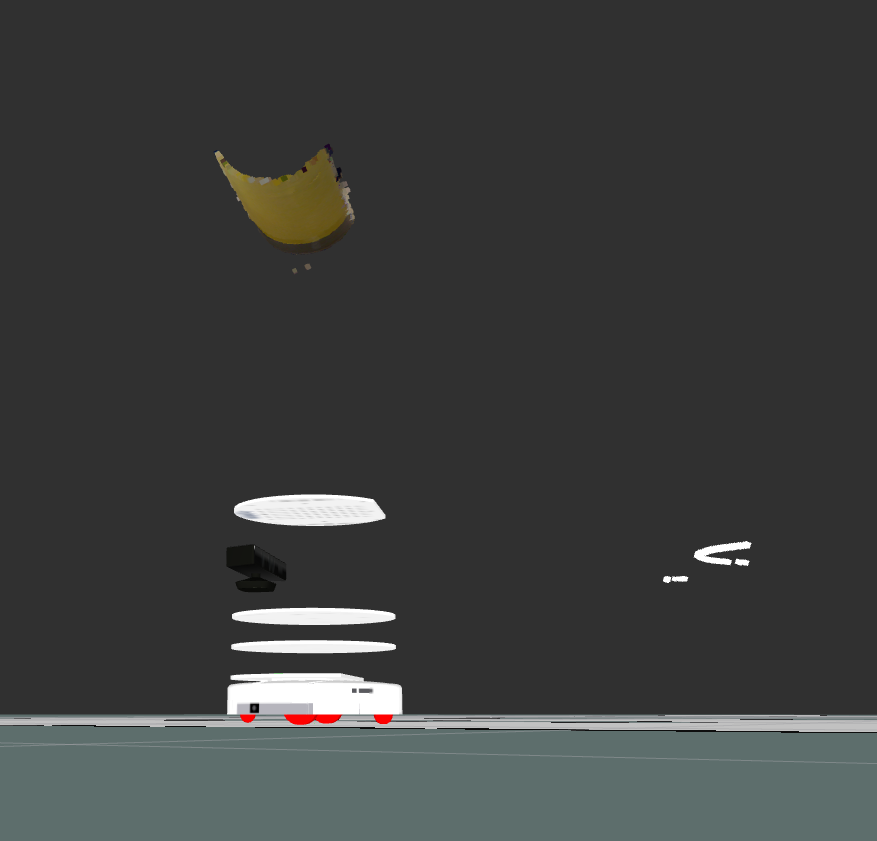
\includegraphics[width=1\textwidth]{cil.png}
  \caption{Slika prikazuje barvne točke detektiranega cilindra.}
  \label{cil}
\end{figure}




\end{document}